% LeNet-5
% Made with Xematics. Positions are in px (1 px = 0.75 pt), as in the SVG export.
\documentclass[tikz, border=4pt]{standalone}
\usepackage{amsmath, amssymb}
\definecolor{xm1}{HTML}{FFFFFF}
\definecolor{xm2}{HTML}{F1F2F4}
\definecolor{xm3}{HTML}{4B5563}
\definecolor{xm4}{HTML}{FBE8C4}
\definecolor{xm5}{HTML}{B97800}
\definecolor{xm6}{HTML}{B8C0CC}
\definecolor{xm7}{HTML}{D4E8F5}
\definecolor{xm8}{HTML}{0072B2}
\definecolor{xm9}{HTML}{DFE3E8}
\definecolor{xm10}{HTML}{AEB3B9}
\definecolor{xm11}{HTML}{6B7280}
\definecolor{xm12}{HTML}{1F2937}
\begin{document}
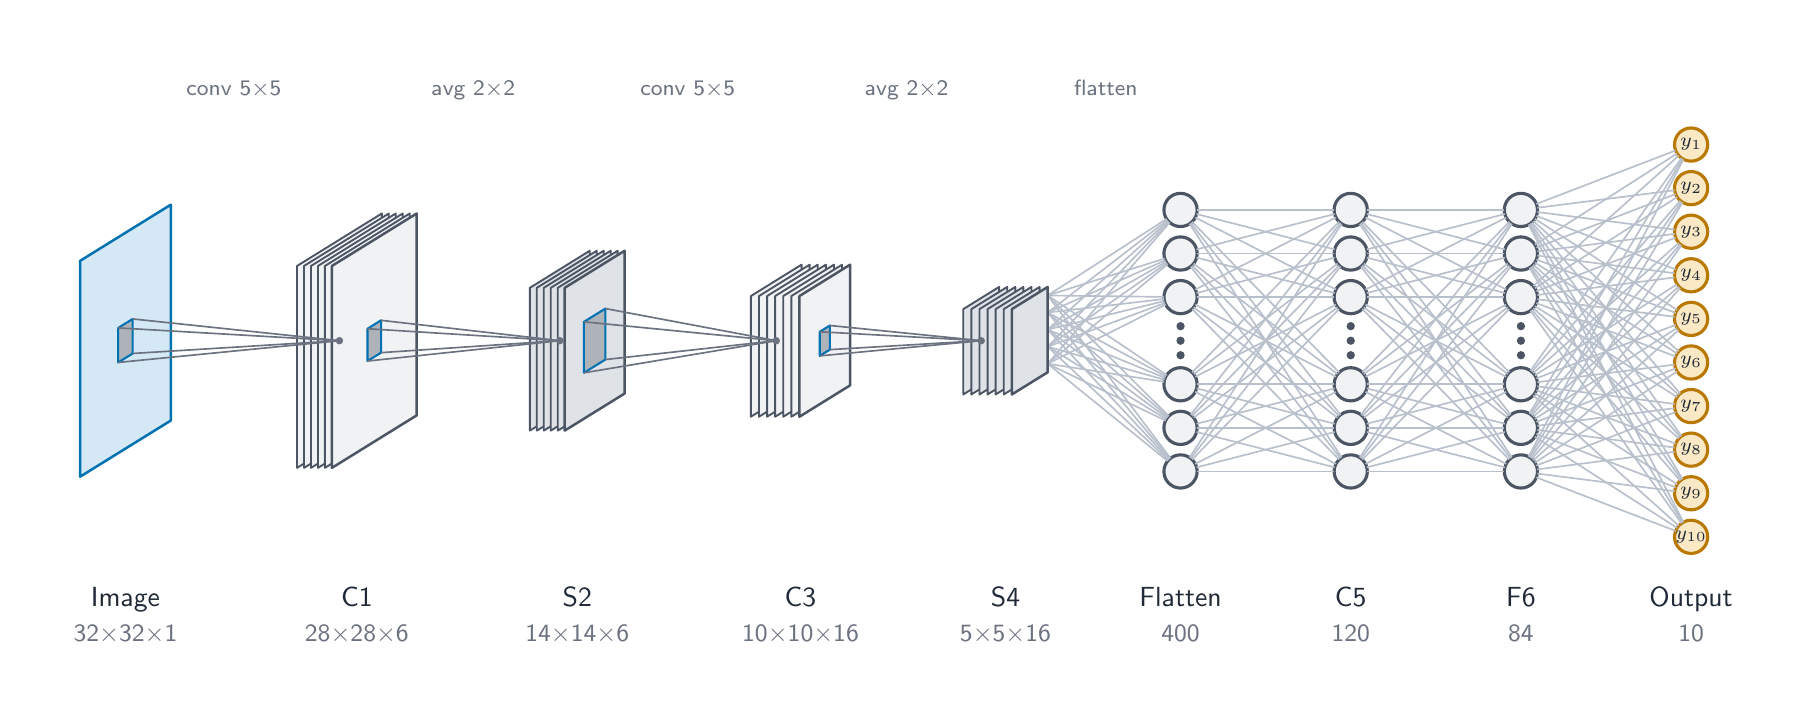
\begin{tikzpicture}[x=0.75pt, y=-0.75pt]
  \tikzset{
    xm hidden/.style={circle, minimum size=12pt, inner sep=0, outer sep=0, fill=xm2, draw=xm3, line width=1.13pt},
    xm output/.style={circle, minimum size=12pt, inner sep=0, outer sep=0, fill=xm4, draw=xm5, line width=1.13pt},
    xm edge/.style={draw=xm6, line width=0.6pt},
    xm map input/.style={fill=xm7, draw=xm8, line width=0.9pt, line join=round},
    xm map hidden back/.style={fill=xm2, draw=xm3, line width=0.68pt, line join=round},
    xm map hidden/.style={fill=xm2, draw=xm3, line width=0.9pt, line join=round},
    xm map pool back/.style={fill=xm9, draw=xm3, line width=0.68pt, line join=round},
    xm map pool/.style={fill=xm9, draw=xm3, line width=0.9pt, line join=round},
    xm dots/.style={fill=xm3},
    xm window/.style={fill=xm10, draw=xm8, line width=0.75pt, line join=round},
    xm ray/.style={draw=xm11, line width=0.6pt},
    xm ray end/.style={fill=xm11},
    xm nodelabel xm12/.style={text=xm12, inner sep=0, font=\sffamily\fontsize{7.5}{9}\selectfont},
    xm name xm12/.style={text=xm12, inner sep=0, font=\sffamily\fontsize{9.75}{11.7}\selectfont},
    xm size xm11/.style={text=xm11, inner sep=0, font=\sffamily\fontsize{9}{10.8}\selectfont},
    xm op xm11/.style={text=xm11, inner sep=0, font=\sffamily\fontsize{8.25}{9.9}\selectfont},
  }
  \fill[xm1] (0,0) rectangle (844.69,320.56);
  % Neurons
  \node[xm hidden] (n-5-0) at (555.44,87.81) {};
  \node[xm hidden] (n-5-1) at (555.44,108.81) {};
  \node[xm hidden] (n-5-2) at (555.44,129.81) {};
  \node[xm hidden] (n-5-397) at (555.44,171.81) {};
  \node[xm hidden] (n-5-398) at (555.44,192.81) {};
  \node[xm hidden] (n-5-399) at (555.44,213.81) {};
  \node[xm hidden] (n-6-0) at (637.44,87.81) {};
  \node[xm hidden] (n-6-1) at (637.44,108.81) {};
  \node[xm hidden] (n-6-2) at (637.44,129.81) {};
  \node[xm hidden] (n-6-117) at (637.44,171.81) {};
  \node[xm hidden] (n-6-118) at (637.44,192.81) {};
  \node[xm hidden] (n-6-119) at (637.44,213.81) {};
  \node[xm hidden] (n-7-0) at (719.44,87.81) {};
  \node[xm hidden] (n-7-1) at (719.44,108.81) {};
  \node[xm hidden] (n-7-2) at (719.44,129.81) {};
  \node[xm hidden] (n-7-81) at (719.44,171.81) {};
  \node[xm hidden] (n-7-82) at (719.44,192.81) {};
  \node[xm hidden] (n-7-83) at (719.44,213.81) {};
  \node[xm output] (n-8-0) at (801.44,56.31) {};
  \node[xm output] (n-8-1) at (801.44,77.31) {};
  \node[xm output] (n-8-2) at (801.44,98.31) {};
  \node[xm output] (n-8-3) at (801.44,119.31) {};
  \node[xm output] (n-8-4) at (801.44,140.31) {};
  \node[xm output] (n-8-5) at (801.44,161.31) {};
  \node[xm output] (n-8-6) at (801.44,182.31) {};
  \node[xm output] (n-8-7) at (801.44,203.31) {};
  \node[xm output] (n-8-8) at (801.44,224.31) {};
  \node[xm output] (n-8-9) at (801.44,245.31) {};
  % Connections 4
  \draw[xm edge] (491.44,129.02) -- (n-5-0);
  \draw[xm edge] (491.44,129.02) -- (n-5-1);
  \draw[xm edge] (491.44,129.02) -- (n-5-2);
  \draw[xm edge] (491.44,129.02) -- (n-5-397);
  \draw[xm edge] (491.44,129.02) -- (n-5-398);
  \draw[xm edge] (491.44,129.02) -- (n-5-399);
  \draw[xm edge] (491.44,137.24) -- (n-5-0);
  \draw[xm edge] (491.44,137.24) -- (n-5-1);
  \draw[xm edge] (491.44,137.24) -- (n-5-2);
  \draw[xm edge] (491.44,137.24) -- (n-5-397);
  \draw[xm edge] (491.44,137.24) -- (n-5-398);
  \draw[xm edge] (491.44,137.24) -- (n-5-399);
  \draw[xm edge] (491.44,145.47) -- (n-5-0);
  \draw[xm edge] (491.44,145.47) -- (n-5-1);
  \draw[xm edge] (491.44,145.47) -- (n-5-2);
  \draw[xm edge] (491.44,145.47) -- (n-5-397);
  \draw[xm edge] (491.44,145.47) -- (n-5-398);
  \draw[xm edge] (491.44,145.47) -- (n-5-399);
  \draw[xm edge] (491.44,153.69) -- (n-5-0);
  \draw[xm edge] (491.44,153.69) -- (n-5-1);
  \draw[xm edge] (491.44,153.69) -- (n-5-2);
  \draw[xm edge] (491.44,153.69) -- (n-5-397);
  \draw[xm edge] (491.44,153.69) -- (n-5-398);
  \draw[xm edge] (491.44,153.69) -- (n-5-399);
  \draw[xm edge] (491.44,161.91) -- (n-5-0);
  \draw[xm edge] (491.44,161.91) -- (n-5-1);
  \draw[xm edge] (491.44,161.91) -- (n-5-2);
  \draw[xm edge] (491.44,161.91) -- (n-5-397);
  \draw[xm edge] (491.44,161.91) -- (n-5-398);
  \draw[xm edge] (491.44,161.91) -- (n-5-399);
  % Connections 5
  \draw[xm edge] (n-5-0) -- (n-6-0);
  \draw[xm edge] (n-5-0) -- (n-6-1);
  \draw[xm edge] (n-5-0) -- (n-6-2);
  \draw[xm edge] (n-5-0) -- (n-6-117);
  \draw[xm edge] (n-5-0) -- (n-6-118);
  \draw[xm edge] (n-5-0) -- (n-6-119);
  \draw[xm edge] (n-5-1) -- (n-6-0);
  \draw[xm edge] (n-5-1) -- (n-6-1);
  \draw[xm edge] (n-5-1) -- (n-6-2);
  \draw[xm edge] (n-5-1) -- (n-6-117);
  \draw[xm edge] (n-5-1) -- (n-6-118);
  \draw[xm edge] (n-5-1) -- (n-6-119);
  \draw[xm edge] (n-5-2) -- (n-6-0);
  \draw[xm edge] (n-5-2) -- (n-6-1);
  \draw[xm edge] (n-5-2) -- (n-6-2);
  \draw[xm edge] (n-5-2) -- (n-6-117);
  \draw[xm edge] (n-5-2) -- (n-6-118);
  \draw[xm edge] (n-5-2) -- (n-6-119);
  \draw[xm edge] (n-5-397) -- (n-6-0);
  \draw[xm edge] (n-5-397) -- (n-6-1);
  \draw[xm edge] (n-5-397) -- (n-6-2);
  \draw[xm edge] (n-5-397) -- (n-6-117);
  \draw[xm edge] (n-5-397) -- (n-6-118);
  \draw[xm edge] (n-5-397) -- (n-6-119);
  \draw[xm edge] (n-5-398) -- (n-6-0);
  \draw[xm edge] (n-5-398) -- (n-6-1);
  \draw[xm edge] (n-5-398) -- (n-6-2);
  \draw[xm edge] (n-5-398) -- (n-6-117);
  \draw[xm edge] (n-5-398) -- (n-6-118);
  \draw[xm edge] (n-5-398) -- (n-6-119);
  \draw[xm edge] (n-5-399) -- (n-6-0);
  \draw[xm edge] (n-5-399) -- (n-6-1);
  \draw[xm edge] (n-5-399) -- (n-6-2);
  \draw[xm edge] (n-5-399) -- (n-6-117);
  \draw[xm edge] (n-5-399) -- (n-6-118);
  \draw[xm edge] (n-5-399) -- (n-6-119);
  % Connections 6
  \draw[xm edge] (n-6-0) -- (n-7-0);
  \draw[xm edge] (n-6-0) -- (n-7-1);
  \draw[xm edge] (n-6-0) -- (n-7-2);
  \draw[xm edge] (n-6-0) -- (n-7-81);
  \draw[xm edge] (n-6-0) -- (n-7-82);
  \draw[xm edge] (n-6-0) -- (n-7-83);
  \draw[xm edge] (n-6-1) -- (n-7-0);
  \draw[xm edge] (n-6-1) -- (n-7-1);
  \draw[xm edge] (n-6-1) -- (n-7-2);
  \draw[xm edge] (n-6-1) -- (n-7-81);
  \draw[xm edge] (n-6-1) -- (n-7-82);
  \draw[xm edge] (n-6-1) -- (n-7-83);
  \draw[xm edge] (n-6-2) -- (n-7-0);
  \draw[xm edge] (n-6-2) -- (n-7-1);
  \draw[xm edge] (n-6-2) -- (n-7-2);
  \draw[xm edge] (n-6-2) -- (n-7-81);
  \draw[xm edge] (n-6-2) -- (n-7-82);
  \draw[xm edge] (n-6-2) -- (n-7-83);
  \draw[xm edge] (n-6-117) -- (n-7-0);
  \draw[xm edge] (n-6-117) -- (n-7-1);
  \draw[xm edge] (n-6-117) -- (n-7-2);
  \draw[xm edge] (n-6-117) -- (n-7-81);
  \draw[xm edge] (n-6-117) -- (n-7-82);
  \draw[xm edge] (n-6-117) -- (n-7-83);
  \draw[xm edge] (n-6-118) -- (n-7-0);
  \draw[xm edge] (n-6-118) -- (n-7-1);
  \draw[xm edge] (n-6-118) -- (n-7-2);
  \draw[xm edge] (n-6-118) -- (n-7-81);
  \draw[xm edge] (n-6-118) -- (n-7-82);
  \draw[xm edge] (n-6-118) -- (n-7-83);
  \draw[xm edge] (n-6-119) -- (n-7-0);
  \draw[xm edge] (n-6-119) -- (n-7-1);
  \draw[xm edge] (n-6-119) -- (n-7-2);
  \draw[xm edge] (n-6-119) -- (n-7-81);
  \draw[xm edge] (n-6-119) -- (n-7-82);
  \draw[xm edge] (n-6-119) -- (n-7-83);
  % Connections 7
  \draw[xm edge] (n-7-0) -- (n-8-0);
  \draw[xm edge] (n-7-0) -- (n-8-1);
  \draw[xm edge] (n-7-0) -- (n-8-2);
  \draw[xm edge] (n-7-0) -- (n-8-3);
  \draw[xm edge] (n-7-0) -- (n-8-4);
  \draw[xm edge] (n-7-0) -- (n-8-5);
  \draw[xm edge] (n-7-0) -- (n-8-6);
  \draw[xm edge] (n-7-0) -- (n-8-7);
  \draw[xm edge] (n-7-0) -- (n-8-8);
  \draw[xm edge] (n-7-0) -- (n-8-9);
  \draw[xm edge] (n-7-1) -- (n-8-0);
  \draw[xm edge] (n-7-1) -- (n-8-1);
  \draw[xm edge] (n-7-1) -- (n-8-2);
  \draw[xm edge] (n-7-1) -- (n-8-3);
  \draw[xm edge] (n-7-1) -- (n-8-4);
  \draw[xm edge] (n-7-1) -- (n-8-5);
  \draw[xm edge] (n-7-1) -- (n-8-6);
  \draw[xm edge] (n-7-1) -- (n-8-7);
  \draw[xm edge] (n-7-1) -- (n-8-8);
  \draw[xm edge] (n-7-1) -- (n-8-9);
  \draw[xm edge] (n-7-2) -- (n-8-0);
  \draw[xm edge] (n-7-2) -- (n-8-1);
  \draw[xm edge] (n-7-2) -- (n-8-2);
  \draw[xm edge] (n-7-2) -- (n-8-3);
  \draw[xm edge] (n-7-2) -- (n-8-4);
  \draw[xm edge] (n-7-2) -- (n-8-5);
  \draw[xm edge] (n-7-2) -- (n-8-6);
  \draw[xm edge] (n-7-2) -- (n-8-7);
  \draw[xm edge] (n-7-2) -- (n-8-8);
  \draw[xm edge] (n-7-2) -- (n-8-9);
  \draw[xm edge] (n-7-81) -- (n-8-0);
  \draw[xm edge] (n-7-81) -- (n-8-1);
  \draw[xm edge] (n-7-81) -- (n-8-2);
  \draw[xm edge] (n-7-81) -- (n-8-3);
  \draw[xm edge] (n-7-81) -- (n-8-4);
  \draw[xm edge] (n-7-81) -- (n-8-5);
  \draw[xm edge] (n-7-81) -- (n-8-6);
  \draw[xm edge] (n-7-81) -- (n-8-7);
  \draw[xm edge] (n-7-81) -- (n-8-8);
  \draw[xm edge] (n-7-81) -- (n-8-9);
  \draw[xm edge] (n-7-82) -- (n-8-0);
  \draw[xm edge] (n-7-82) -- (n-8-1);
  \draw[xm edge] (n-7-82) -- (n-8-2);
  \draw[xm edge] (n-7-82) -- (n-8-3);
  \draw[xm edge] (n-7-82) -- (n-8-4);
  \draw[xm edge] (n-7-82) -- (n-8-5);
  \draw[xm edge] (n-7-82) -- (n-8-6);
  \draw[xm edge] (n-7-82) -- (n-8-7);
  \draw[xm edge] (n-7-82) -- (n-8-8);
  \draw[xm edge] (n-7-82) -- (n-8-9);
  \draw[xm edge] (n-7-83) -- (n-8-0);
  \draw[xm edge] (n-7-83) -- (n-8-1);
  \draw[xm edge] (n-7-83) -- (n-8-2);
  \draw[xm edge] (n-7-83) -- (n-8-3);
  \draw[xm edge] (n-7-83) -- (n-8-4);
  \draw[xm edge] (n-7-83) -- (n-8-5);
  \draw[xm edge] (n-7-83) -- (n-8-6);
  \draw[xm edge] (n-7-83) -- (n-8-7);
  \draw[xm edge] (n-7-83) -- (n-8-8);
  \draw[xm edge] (n-7-83) -- (n-8-9);
  % Layers
  \draw[xm map input] (25.27,112.33) -- (68.95,85.29) -- (68.95,189.29) -- (25.27,216.33) -- cycle;
  \draw[xm map hidden back] (129.77,114.81) -- (170.63,89.52) -- (170.63,186.8) -- (129.77,212.1) -- cycle;
  \draw[xm map hidden back] (133.13,114.81) -- (173.99,89.52) -- (173.99,186.8) -- (133.13,212.1) -- cycle;
  \draw[xm map hidden back] (136.49,114.81) -- (177.35,89.52) -- (177.35,186.8) -- (136.49,212.1) -- cycle;
  \draw[xm map hidden back] (139.85,114.81) -- (180.7,89.52) -- (180.7,186.8) -- (139.85,212.1) -- cycle;
  \draw[xm map hidden back] (143.2,114.81) -- (184.06,89.52) -- (184.06,186.8) -- (143.2,212.1) -- cycle;
  \draw[xm map hidden] (146.56,114.81) -- (187.42,89.52) -- (187.42,186.8) -- (146.56,212.1) -- cycle;
  \draw[xm map pool back] (241.94,125.36) -- (270.83,107.47) -- (270.83,176.26) -- (241.94,194.15) -- cycle;
  \draw[xm map pool back] (245.29,125.36) -- (274.19,107.47) -- (274.19,176.26) -- (245.29,194.15) -- cycle;
  \draw[xm map pool back] (248.65,125.36) -- (277.54,107.47) -- (277.54,176.26) -- (248.65,194.15) -- cycle;
  \draw[xm map pool back] (252.01,125.36) -- (280.9,107.47) -- (280.9,176.26) -- (252.01,194.15) -- cycle;
  \draw[xm map pool back] (255.37,125.36) -- (284.26,107.47) -- (284.26,176.26) -- (255.37,194.15) -- cycle;
  \draw[xm map pool] (258.72,125.36) -- (287.61,107.47) -- (287.61,176.26) -- (258.72,194.15) -- cycle;
  \draw[xm map hidden back] (348.44,129.3) -- (372.86,114.18) -- (372.86,172.32) -- (348.44,187.44) -- cycle;
  \draw[xm map hidden back] (352.34,129.3) -- (376.76,114.18) -- (376.76,172.32) -- (352.34,187.44) -- cycle;
  \draw[xm map hidden back] (356.24,129.3) -- (380.66,114.18) -- (380.66,172.32) -- (356.24,187.44) -- cycle;
  \draw[xm map hidden back] (360.14,129.3) -- (384.56,114.18) -- (384.56,172.32) -- (360.14,187.44) -- cycle;
  \draw[xm map hidden back] (364.04,129.3) -- (388.46,114.18) -- (388.46,172.32) -- (364.04,187.44) -- cycle;
  \draw[xm map hidden back] (367.94,129.3) -- (392.36,114.18) -- (392.36,172.32) -- (367.94,187.44) -- cycle;
  \draw[xm map hidden] (371.84,129.3) -- (396.26,114.18) -- (396.26,172.32) -- (371.84,187.44) -- cycle;
  \draw[xm map pool back] (450.77,135.6) -- (468.04,124.91) -- (468.04,166.02) -- (450.77,176.71) -- cycle;
  \draw[xm map pool back] (454.67,135.6) -- (471.94,124.91) -- (471.94,166.02) -- (454.67,176.71) -- cycle;
  \draw[xm map pool back] (458.57,135.6) -- (475.84,124.91) -- (475.84,166.02) -- (458.57,176.71) -- cycle;
  \draw[xm map pool back] (462.47,135.6) -- (479.74,124.91) -- (479.74,166.02) -- (462.47,176.71) -- cycle;
  \draw[xm map pool back] (466.37,135.6) -- (483.64,124.91) -- (483.64,166.02) -- (466.37,176.71) -- cycle;
  \draw[xm map pool back] (470.27,135.6) -- (487.54,124.91) -- (487.54,166.02) -- (470.27,176.71) -- cycle;
  \draw[xm map pool] (474.17,135.6) -- (491.44,124.91) -- (491.44,166.02) -- (474.17,176.71) -- cycle;
  \fill[xm dots] (555.44,143.81) circle[radius=2];
  \fill[xm dots] (555.44,150.81) circle[radius=2];
  \fill[xm dots] (555.44,157.81) circle[radius=2];
  \fill[xm dots] (637.44,143.81) circle[radius=2];
  \fill[xm dots] (637.44,150.81) circle[radius=2];
  \fill[xm dots] (637.44,157.81) circle[radius=2];
  \fill[xm dots] (719.44,143.81) circle[radius=2];
  \fill[xm dots] (719.44,150.81) circle[radius=2];
  \fill[xm dots] (719.44,157.81) circle[radius=2];
  \draw[xm window] (43.62,144.65) -- (50.6,140.33) -- (50.6,156.97) -- (43.62,161.29) -- cycle;
  \draw[xm ray] (43.62,144.65) -- (150.2,150.81);
  \draw[xm ray] (50.6,140.33) -- (150.2,150.81);
  \draw[xm ray] (50.6,156.97) -- (150.2,150.81);
  \draw[xm ray] (43.62,161.29) -- (150.2,150.81);
  \fill[xm ray end] (150.2,150.81) circle[radius=1.8];
  \draw[xm window] (163.72,145.05) -- (170.26,141) -- (170.26,156.57) -- (163.72,160.62) -- cycle;
  \draw[xm ray] (163.72,145.05) -- (256.38,150.81);
  \draw[xm ray] (170.26,141) -- (256.38,150.81);
  \draw[xm ray] (170.26,156.57) -- (256.38,150.81);
  \draw[xm ray] (163.72,160.62) -- (256.38,150.81);
  \fill[xm ray end] (256.38,150.81) circle[radius=1.8];
  \draw[xm window] (268.01,141.72) -- (278.33,135.33) -- (278.33,159.9) -- (268.01,166.29) -- cycle;
  \draw[xm ray] (268.01,141.72) -- (360.65,150.81);
  \draw[xm ray] (278.33,135.33) -- (360.65,150.81);
  \draw[xm ray] (278.33,159.9) -- (360.65,150.81);
  \draw[xm ray] (268.01,166.29) -- (360.65,150.81);
  \fill[xm ray end] (360.65,150.81) circle[radius=1.8];
  \draw[xm window] (381.61,146.51) -- (386.49,143.48) -- (386.49,155.11) -- (381.61,158.13) -- cycle;
  \draw[xm ray] (381.61,146.51) -- (459.41,150.81);
  \draw[xm ray] (386.49,143.48) -- (459.41,150.81);
  \draw[xm ray] (386.49,155.11) -- (459.41,150.81);
  \draw[xm ray] (381.61,158.13) -- (459.41,150.81);
  \fill[xm ray end] (459.41,150.81) circle[radius=1.8];
  % Labels
  \node[xm nodelabel xm12, anchor=center] at (801.44,56.31) {$y_{1}$};
  \node[xm nodelabel xm12, anchor=center] at (801.44,77.31) {$y_{2}$};
  \node[xm nodelabel xm12, anchor=center] at (801.44,98.31) {$y_{3}$};
  \node[xm nodelabel xm12, anchor=center] at (801.44,119.31) {$y_{4}$};
  \node[xm nodelabel xm12, anchor=center] at (801.44,140.31) {$y_{5}$};
  \node[xm nodelabel xm12, anchor=center] at (801.44,161.31) {$y_{6}$};
  \node[xm nodelabel xm12, anchor=center] at (801.44,182.31) {$y_{7}$};
  \node[xm nodelabel xm12, anchor=center] at (801.44,203.31) {$y_{8}$};
  \node[xm nodelabel xm12, anchor=center] at (801.44,224.31) {$y_{9}$};
  \node[xm nodelabel xm12, anchor=center] at (801.44,245.31) {$y_{10}$};
  \node[xm name xm12, anchor=base] at (47.11,278.9) {Image};
  \node[xm size xm11, anchor=base] at (47.11,295.66) {32\ensuremath{\times}32\ensuremath{\times}1};
  \node[xm op xm11, anchor=base] at (99.36,32.66) {conv 5\ensuremath{\times}5};
  \node[xm name xm12, anchor=base] at (158.6,278.9) {C1};
  \node[xm size xm11, anchor=base] at (158.6,295.66) {28\ensuremath{\times}28\ensuremath{\times}6};
  \node[xm op xm11, anchor=base] at (214.68,32.66) {avg 2\ensuremath{\times}2};
  \node[xm name xm12, anchor=base] at (264.78,278.9) {S2};
  \node[xm size xm11, anchor=base] at (264.78,295.66) {14\ensuremath{\times}14\ensuremath{\times}6};
  \node[xm op xm11, anchor=base] at (318.03,32.66) {conv 5\ensuremath{\times}5};
  \node[xm name xm12, anchor=base] at (372.35,278.9) {C3};
  \node[xm size xm11, anchor=base] at (372.35,295.66) {10\ensuremath{\times}10\ensuremath{\times}16};
  \node[xm op xm11, anchor=base] at (423.51,32.66) {avg 2\ensuremath{\times}2};
  \node[xm name xm12, anchor=base] at (471.11,278.9) {S4};
  \node[xm size xm11, anchor=base] at (471.11,295.66) {5\ensuremath{\times}5\ensuremath{\times}16};
  \node[xm op xm11, anchor=base] at (519.44,32.66) {flatten};
  \node[xm name xm12, anchor=base] at (555.44,278.9) {Flatten};
  \node[xm size xm11, anchor=base] at (555.44,295.66) {400};
  \node[xm name xm12, anchor=base] at (637.44,278.9) {C5};
  \node[xm size xm11, anchor=base] at (637.44,295.66) {120};
  \node[xm name xm12, anchor=base] at (719.44,278.9) {F6};
  \node[xm size xm11, anchor=base] at (719.44,295.66) {84};
  \node[xm name xm12, anchor=base] at (801.44,278.9) {Output};
  \node[xm size xm11, anchor=base] at (801.44,295.66) {10};
\end{tikzpicture}
\end{document}
